\documentclass[12pt]{article}

% 基础宏包
\usepackage{graphicx}  % 插入图片
\usepackage[english]{babel}  % 英语语言支持
% \usepackage[UTF8]{ctex}  % 如果不需要中文，可以注释掉这一行

% 数学宏包
\usepackage{amsmath}  % 数学排版增强
\usepackage{amsfonts} % 数学字体

% 图表相关
\usepackage{float}    % 浮动体控制 [H] 选项
\usepackage{tikz}     % 绘图
\usepackage{pgfplots} % 函数绘图
\pgfplotsset{compat=1.18} % 设置pgfplots兼容性

% 页面设置
\usepackage{geometry}
\geometry{
  a4paper,
  left=2cm,
  right=2cm,
  top=2cm,
  bottom=2cm
}

% 版式设置
\usepackage{fancyhdr}    % 页眉页脚
\usepackage{lastpage}    % 最后一页引用
\usepackage{multicol}    % 多栏排版
\usepackage{tabularx}    % 表格增强

% 文本修饰
\usepackage{ulem}        % 下划线等
\usepackage{enumitem}    % 列表样式
\usepackage{titlesec}    % 标题样式
\usepackage[export]{adjustbox} % 图片对齐

% 颜色
\usepackage{color}       % 颜色支持

\linespread{1.5}         % 1.5倍行距

\title{Lab 3}
\author{Emilien Zhang}
\date{7 April 2026}

\begin{document}

\maketitle

\section*{Problem 1}

\subsection*{(a)}
\begin{figure}[H]
  \centering
  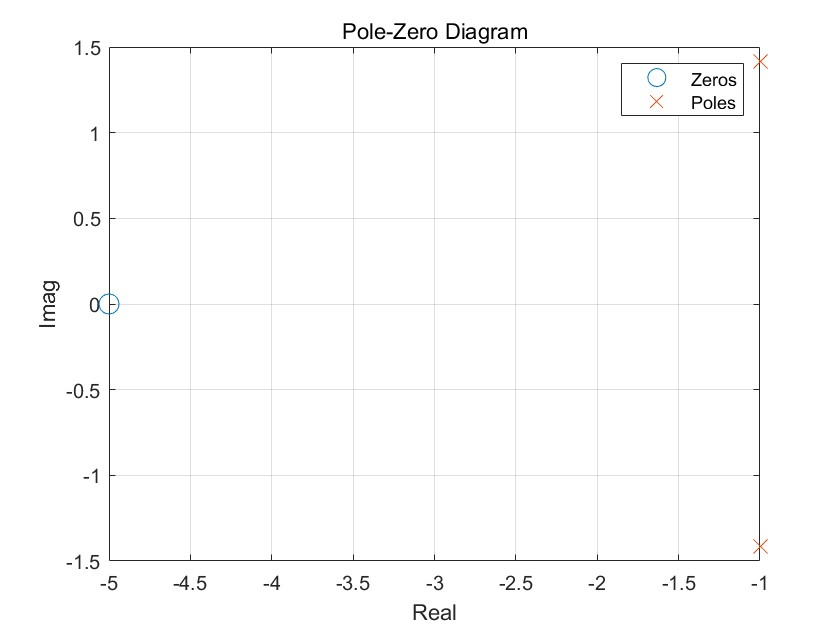
\includegraphics[width=0.5\textwidth]{11.jpg}
  
\end{figure}

\begin{figure}[H]
  \centering
  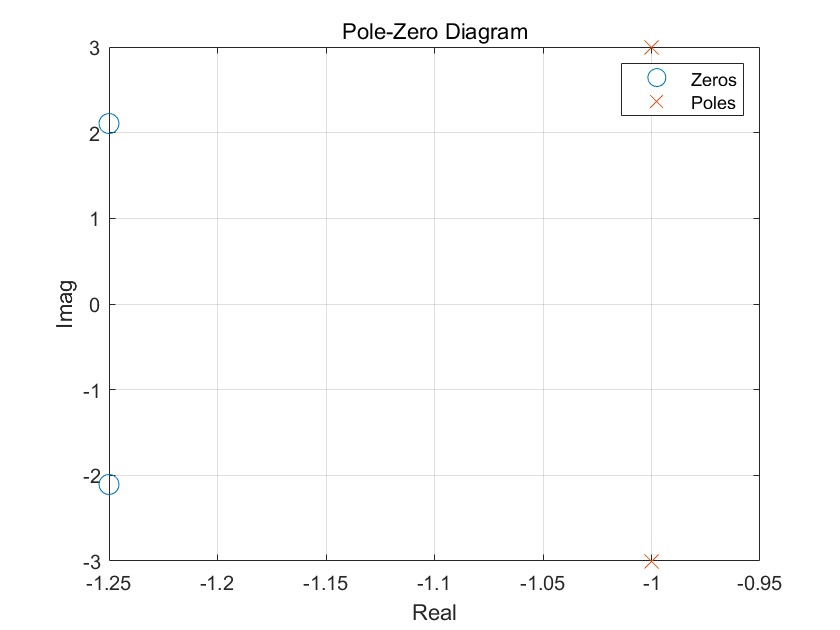
\includegraphics[width=0.5\textwidth]{12.jpg}
  
\end{figure}

\begin{figure}[H]
  \centering
  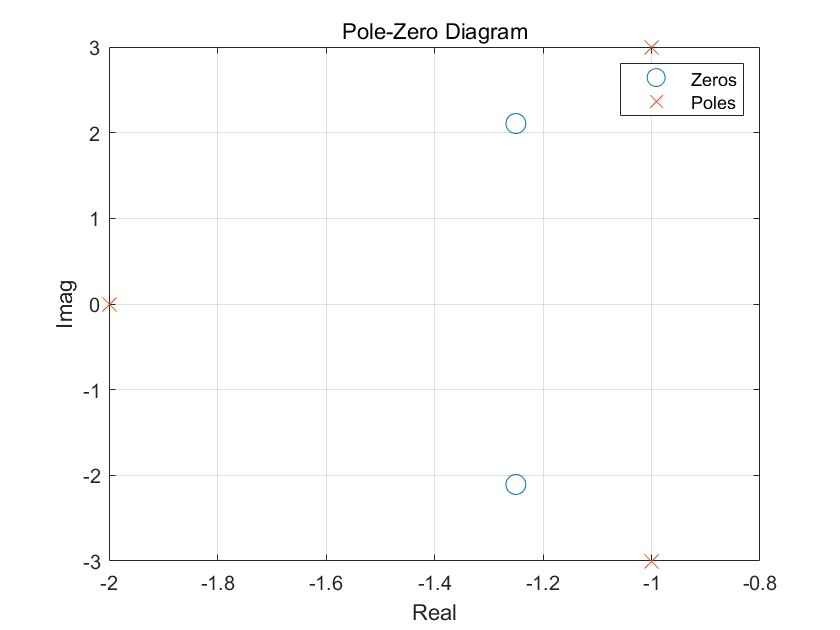
\includegraphics[width=0.5\textwidth]{13.jpg}
  
\end{figure}

\subsection*{(b)}
\subsubsection*{(i)}
Since \(H(s) = \dfrac{s+5}{s^2 + 2s + 3}\) , we have \boxed{zeros} \(s=-5\) and \boxed{poles} \(s=-1 \pm \sqrt{2}i\) .

for a stable system, ROC must includethe entire imaginart axis, so ROC is \(Re(s)>-1\) . 


\subsubsection*{(ii)}
Since \(H(s) = \dfrac{2s^2+5s+12}{s^2 + 2s + 10}\) , we have \boxed{zeros} \(s=\dfrac{-5\pm \sqrt{71}i}{4}\) and \boxed{poles} \(s=-1 \pm 3i\) .

for a stable system, ROC must includethe entire imaginart axis, so ROC is \(Re(s)>-1\) . 


\subsubsection*{(iii)}
Since \(H(s) = \dfrac{2s^2+5s+12}{(s^2 + 2s + 10)(s + 2)}\) , we have \boxed{zeros} \(s=\dfrac{-5\pm \sqrt{71}i}{4}\) and \boxed{poles} \(s=-1 \pm 3i,s=-2\) .

for a stable system, ROC must includethe entire imaginart axis, so ROC is \(Re(s)>-1\) . 

\subsection*{(c)}

Diff.eq for the casual LTI system is
\[\frac{\mathrm{d}y(t)}{\mathrm{d}t} - 3y(t) = \frac{\mathrm{d}^2x(t)}{\mathrm{d}t} + 2\frac{\mathrm{d}x(t)}{\mathrm{d}t} + 5x(t)\]

Laplace Transforms of the diff.eq are
\[sY(s) - 3Y(s) = s^2 X(s) + 2s X(s) + 5X(s)\]
or
\[H(s)=\frac{Y(s)}{X(s)} = \frac{s^2 + 2s + 5}{s-3}\]

\begin{figure}[H]
  \centering
  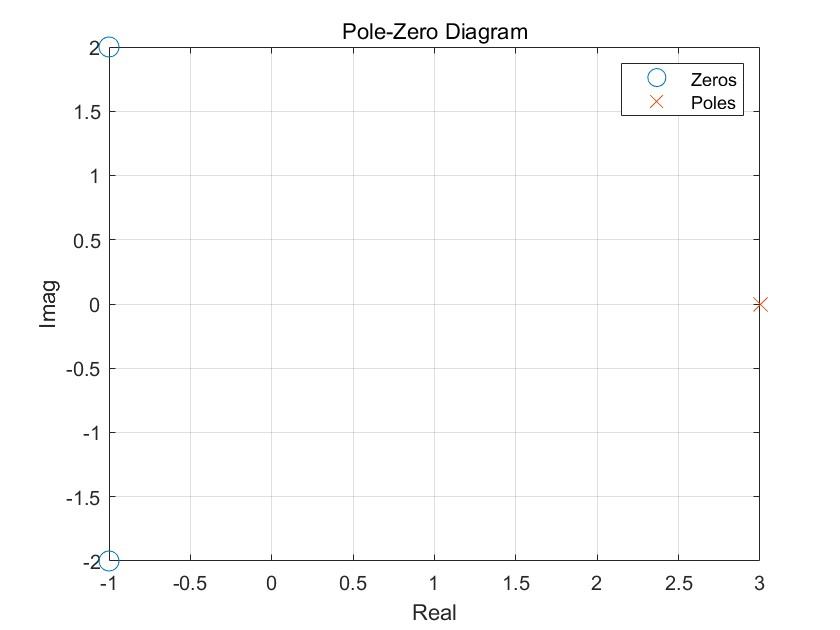
\includegraphics[width=0.5\textwidth]{14.jpg}
 
\end{figure}

we have \boxed{zeros} \(s=-1 \pm 2i\) and \boxed{poles} \(s=3\) .


\subsection*{(d)}
The function \texttt{pzplot(b,a,ROC)} (where \texttt{ROC} is a point in the ROC) determines the region of convergence as follows:

\begin{enumerate}
    \item Compute all poles of $H(s)$ using \texttt{roots(a)}.
    \item Compare the real part of each pole with $\Re(s_0)$, where $s_0$ is the user-provided \texttt{ROC} point.
    \item If any poles satisfy $\Re(p_i) < \Re(s_0)$ (poles to the left), find the left boundary as $\ell = \max\{\Re(p_i) \mid \Re(p_i) < \Re(s_0)\}$. Draw a vertical dashed line at $\Re(s) = \ell$.
    \item If any poles satisfy $\Re(p_i) > \Re(s_0)$ (poles to the right), find the right boundary as $r = \min\{\Re(p_i) \mid \Re(p_i) > \Re(s_0)\}$. Draw a vertical dashed line at $\Re(s) = r$.
    \item The ROC is the vertical strip containing $s_0$: $\ell < \Re(s) < r$ (if no poles on a side, that boundary is $\pm\infty$).
\end{enumerate}

This works because the ROC of a rational Laplace transform is always a vertical strip bounded by the real parts of poles and contains no poles.

\section*{Problem 2}

\subsection*{(a)}
\begin{figure}[H]
  \centering
  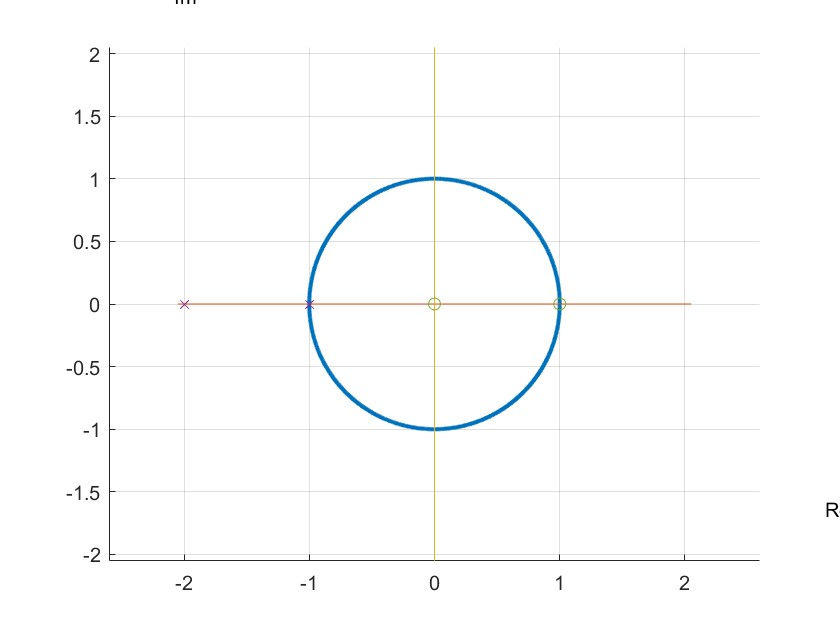
\includegraphics[width=0.5\textwidth]{21.jpg}
 
    \end{figure}

\subsection*{(b)}
\[
y[n] + y[n-1] + 0.5y[n-2] = x[n]
\]

Taking the Z-transform of both sides (assuming zero initial conditions):
\[
Y(z) + z^{-1}Y(z) + 0.5z^{-2}Y(z) = X(z)
\]

Factor out \(Y(z)\):
\[
Y(z)\left(1 + z^{-1} + 0.5z^{-2}\right) = X(z)
\]

Thus, the system function is:
\[
H(z) = \frac{Y(z)}{X(z)} = \frac{1}{1 + z^{-1} + 0.5z^{-2}}
\]

\begin{figure}[H]
  \centering
  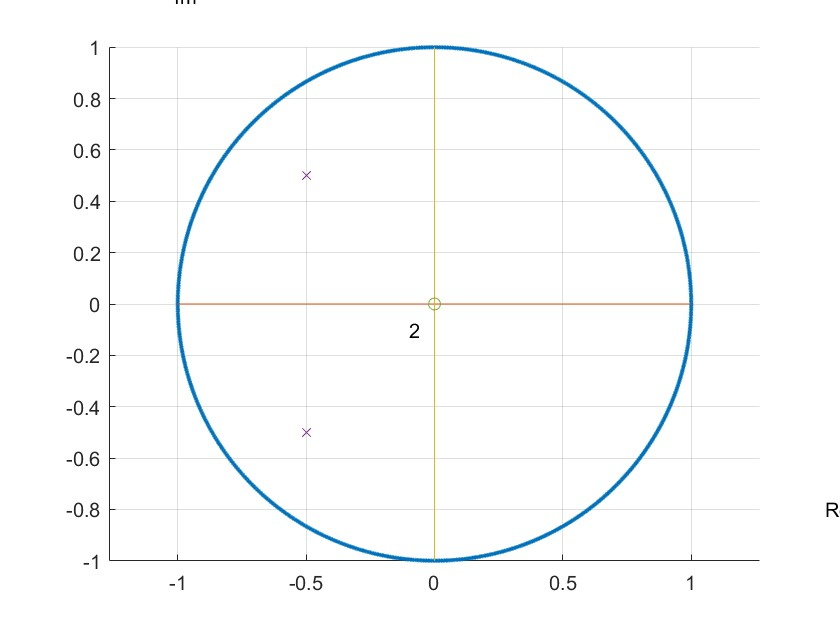
\includegraphics[width=0.5\textwidth]{22.jpg}
  
\end{figure}


\subsection*{(c)}
\[
y[n] - 1.25y[n-1] + 0.75y[n-2] - 0.125y[n-3] = x[n] + 0.5x[n-1]
\]

Taking the Z-transform:
\[
Y(z) - 1.25z^{-1}Y(z) + 0.75z^{-2}Y(z) - 0.125z^{-3}Y(z) = X(z) + 0.5z^{-1}X(z)
\]

Factor out \(Y(z)\) and \(X(z)\):
\[
Y(z)\left(1 - 1.25z^{-1} + 0.75z^{-2} - 0.125z^{-3}\right) = X(z)\left(1 + 0.5z^{-1}\right)
\]

Thus, the system function is:
\[
H(z) = \frac{Y(z)}{X(z)} = \frac{1 + 0.5z^{-1}}{1 - 1.25z^{-1} + 0.75z^{-2} - 0.125z^{-3}}
\]



\begin{figure}[H]
  \centering
  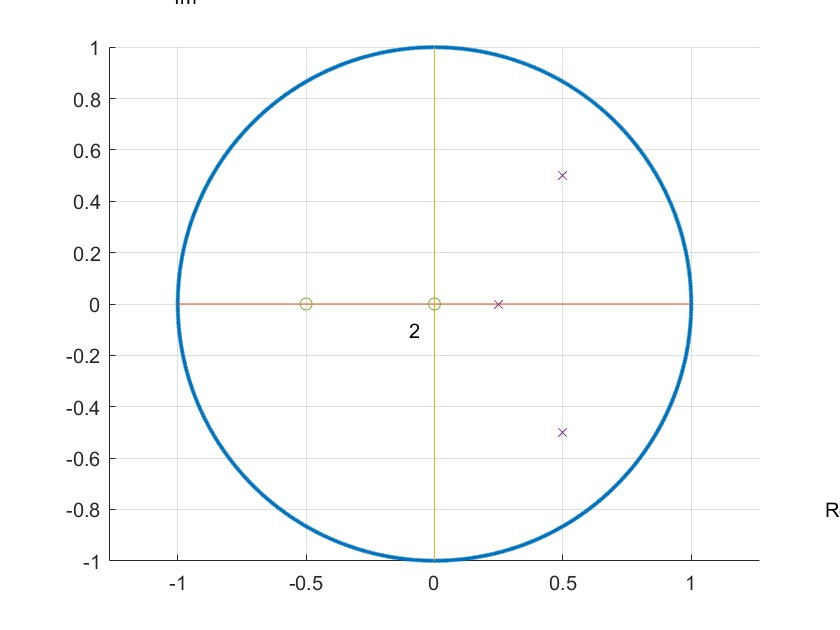
\includegraphics[width=0.5\textwidth]{23.jpg}
 
\end{figure}


\section*{Problem 3}


\subsection*{(a)}

The original differential equation (9.11) has system function:
\[
H_{ac}(s) = \frac{\sum_{m=0}^{M} b_m s^m}{\sum_{k=0}^{K} a_k s^k}.
\]

The time-reversed differential equation (9.12) (substituting $t \to -t$) has system function:
\[
H_c(s) = \frac{\sum_{m=0}^{M} (-1)^m b_m s^m}{\sum_{k=0}^{K} (-1)^k a_k s^k}
      = \frac{\sum_{m=0}^{M} b_m (-s)^m}{\sum_{k=0}^{K} a_k (-s)^k}
      = H_{ac}(-s).
\]

Thus:
\begin{itemize}
    \item \textbf{Pole relationship:} If $p$ is a pole of $H_{ac}(s)$, then $-p$ is a pole of $H_c(s)$. The poles are symmetric about the origin (both real and imaginary parts change sign).
    \item \textbf{System function relationship:} $H_c(s) = H_{ac}(-s)$.
\end{itemize}
\subsection*{(b)(c)}

Diff.eq is 
\[\frac{dy(t)}{dt} + 2y(t) = x(t)\]

The laplace transform is 
\[sY(s)+2Y(s)=X(s)\]
or
\[H(s)=\frac{Y(s)}{X(s)}=\frac{1}{s+2}\]
The impulse response is \(h(t)=e^{-2t}u(t)\) , ROC is \(Re(s)>-2\)(casual) .

Or \(h(t)=-e^{-2t}u(-t)\) , ROC is \(Re(s)<-2\)(anticausal) .

\subsection*{(d)}
\begin{figure}[H]
  \centering
  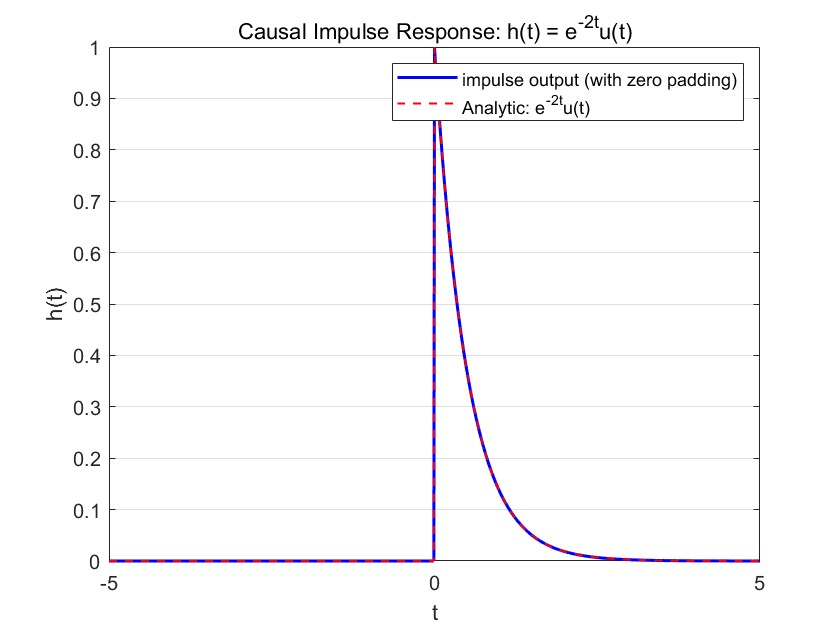
\includegraphics[width=0.5\textwidth]{31.jpg}
 
  \end{figure}

\subsection*{(e)}
\begin{figure}[H]
  \centering
  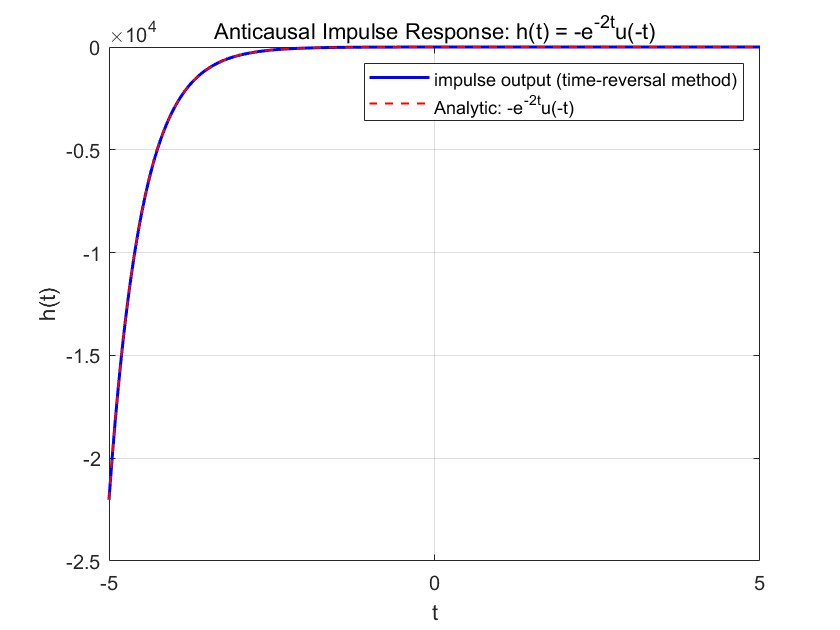
\includegraphics[width=0.5\textwidth]{32.jpg}

  \end{figure}

\subsection*{(f)}

Given:
\begin{itemize}
    \item $h(t) = -e^{-2t}u(-t)$
    \item $x(t) = e^{5t/2}u(-t)$
\end{itemize}

The output is $y(t) = h(t) * x(t) = \int_{-\infty}^{\infty} h(\tau)x(t-\tau)d\tau$.

For $t > 0$, the convolution yields $y(t) = 0$ because the integrand is zero.

For $t \leq 0$:
\begin{align*}
y(t) &= \int_{\tau=t}^{0} \left[-e^{-2\tau}\right] \cdot \left[e^{5(t-\tau)/2}\right] d\tau \\
&= -e^{5t/2} \int_{t}^{0} e^{-2\tau - 5\tau/2} d\tau \\
&= -e^{5t/2} \int_{t}^{0} e^{-9\tau/2} d\tau \\
&= -e^{5t/2} \left[ -\frac{2}{9} e^{-9\tau/2} \right]_{t}^{0} \\
&= -e^{5t/2} \cdot \left(-\frac{2}{9}\right) \left(1 - e^{-9t/2}\right) \\
&= \frac{2}{9} e^{5t/2} \left(1 - e^{-9t/2}\right) \\
&= \frac{2}{9} \left(e^{5t/2} - e^{-2t}\right)
\end{align*}

Therefore:
\[
\boxed{y(t) = \frac{2}{9}\left(e^{5t/2} - e^{-2t}\right) u(-t)}
\]

\subsection*{(g)}

\begin{figure}[H]
    \centering
    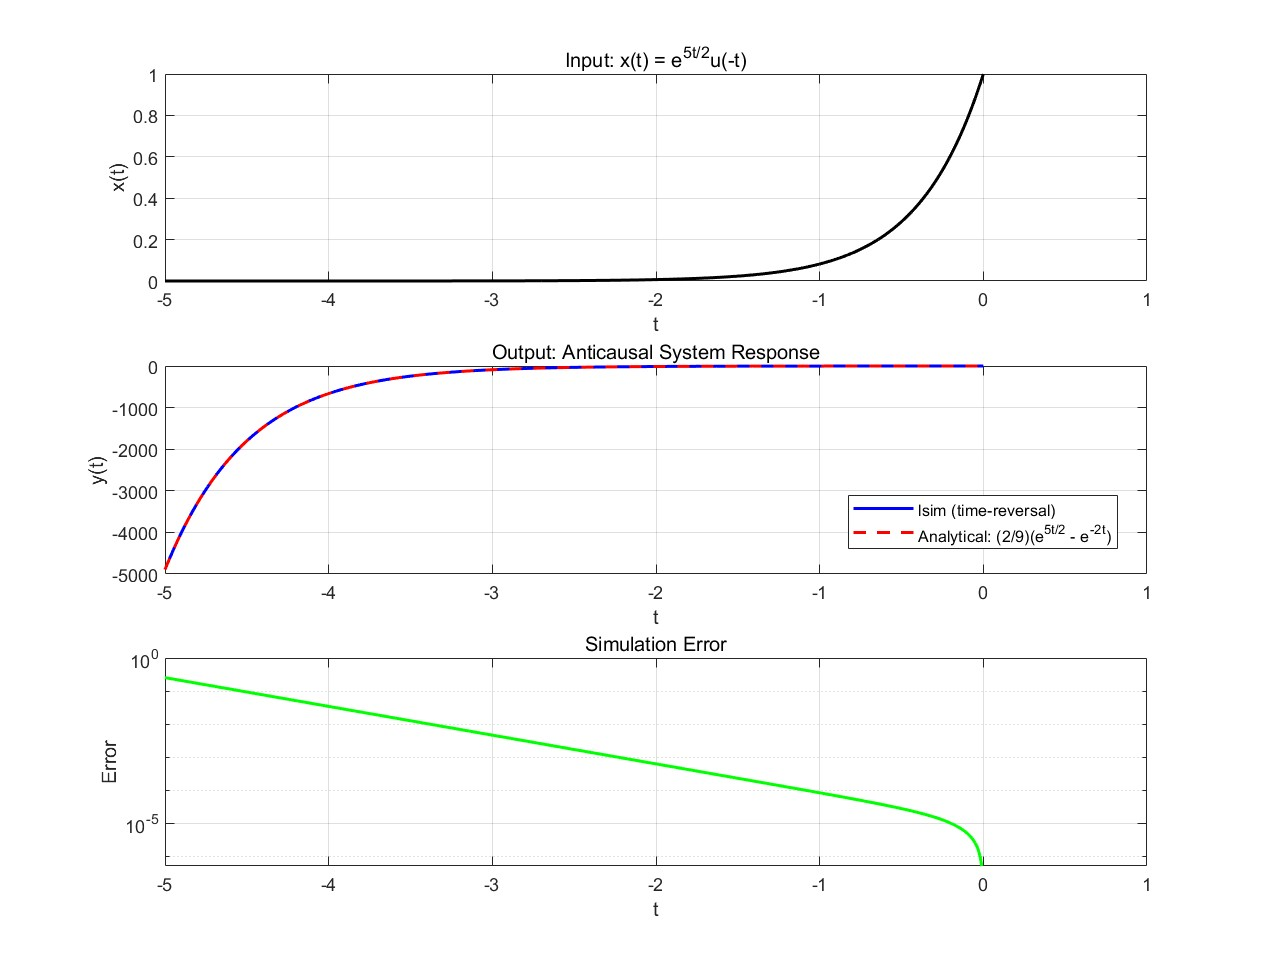
\includegraphics[width=1\textwidth]{33.jpg}
  
\end{figure}

\subsection*{(h)}

The system function is:
\[
H(s) = \frac{s^2 + 7s + 21}{s^3 + s^2 + 24s - 26}
\]

\textbf{Poles and Zeros:}
\begin{itemize}
    \item Zeros: $s = -3.5 \pm j2.78$ (from $s^2 + 7s + 21 = 0$)
    \item Poles: $s \approx 1$, $s \approx -1 \pm j5$ (from $s^3 + s^2 + 24s - 26 = 0$)
\end{itemize}

\textbf{Possible ROCs:}
\begin{enumerate}
    \item $\Re(s) > 1$ (causal, UNSTABLE)
    \item $-1 < \Re(s) < 1$ (noncausal, STABLE)
    \item $\Re(s) < -1$ (anticausal, UNSTABLE)
\end{enumerate}

\textbf{Stable system ROC:} $-1 < \Re(s) < 1$ (vertical strip containing the imaginary axis).

\begin{figure}[H]
\centering
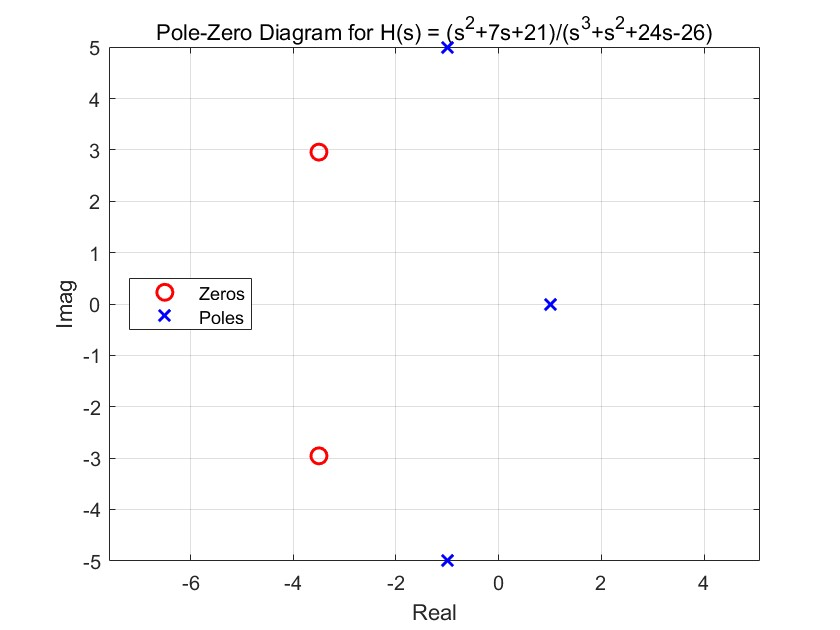
\includegraphics[width=0.5\textwidth]{34.jpg}
\end{figure}


\subsection*{(i)}

Using \texttt{residue}:
\[
H(s) = \frac{r_1}{s - p_1} + \frac{r_2}{s - p_2} + \frac{r_3}{s - p_3}
\]
where $p_1 \approx 1$, $p_{2,3} \approx -1 \pm j5$, and $r_i$ are the corresponding residues.

\textbf{Impulse responses for each ROC:}
\begin{itemize}
    \item ROC: $\Re(s) > 1$ (causal, unstable):
    \[
    h(t) = \left( r_1 e^{p_1 t} + r_2 e^{p_2 t} + r_3 e^{p_3 t} \right) u(t)
    \]
    
    \item ROC: $-1 < \Re(s) < 1$ (stable, noncausal):
    \[
    h(t) = r_1 e^{p_1 t} u(-t) + \left( r_2 e^{p_2 t} + r_3 e^{p_3 t} \right) u(t)
    \]
    
    \item ROC: $\Re(s) < -1$ (anticausal, unstable):
    \[
    h(t) = -\left( r_1 e^{p_1 t} + r_2 e^{p_2 t} + r_3 e^{p_3 t} \right) u(-t)
    \]
\end{itemize}

\subsection*{(j)}

The causal system corresponds to ROC $\Re(s) > 1$. Using \texttt{impulse(b,a,ts)}:

\begin{figure}[H]
\centering
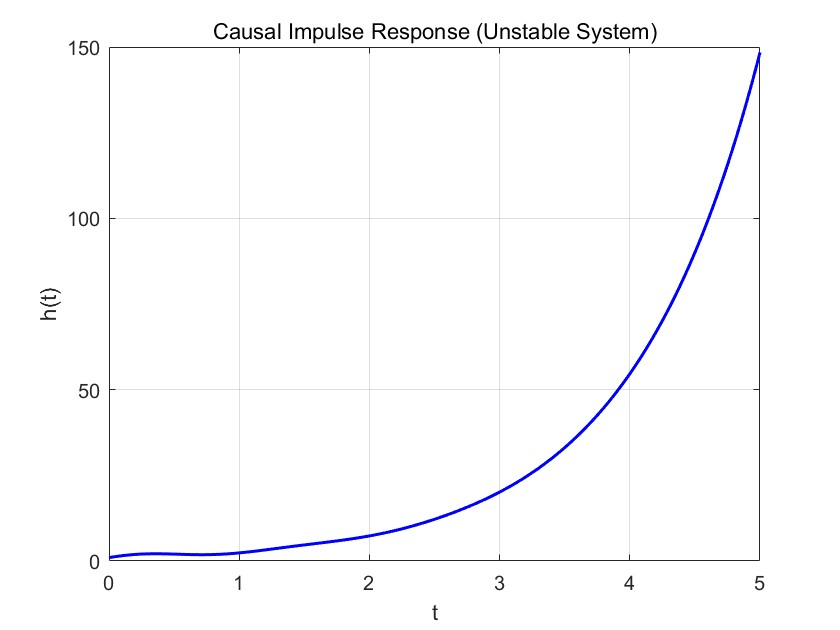
\includegraphics[width=0.5\textwidth]{35.jpg}
\end{figure}


\textbf{Auxiliary conditions for causal system:} Initial rest conditions: $y(t) = 0$ and all derivatives zero for $t < t_0$.

\subsection*{(k)}

The anticausal system corresponds to ROC $\Re(s) < -1$. Using time-reversal method:
\begin{enumerate}
    \item Time-reverse the differential equation to obtain a causal system:
    \[
    H_c(s) = H(-s) = \frac{s^2 - 7s + 21}{-s^3 + s^2 - 24s - 26}
    \]
    \item Multiply numerator and denominator by $-1$ to make leading coefficient positive.
    \item Compute impulse response $w(t)$ of the causal system using \texttt{impulse}.
    \item Time-reverse to get $h_{\text{anticausal}}(t) = w(-t)$.
\end{enumerate}

\textbf{Auxiliary conditions for anticausal system:} Final rest conditions: $y(t) = 0$ and all derivatives zero for $t > t_0$.

\begin{figure}[H]
  \centering
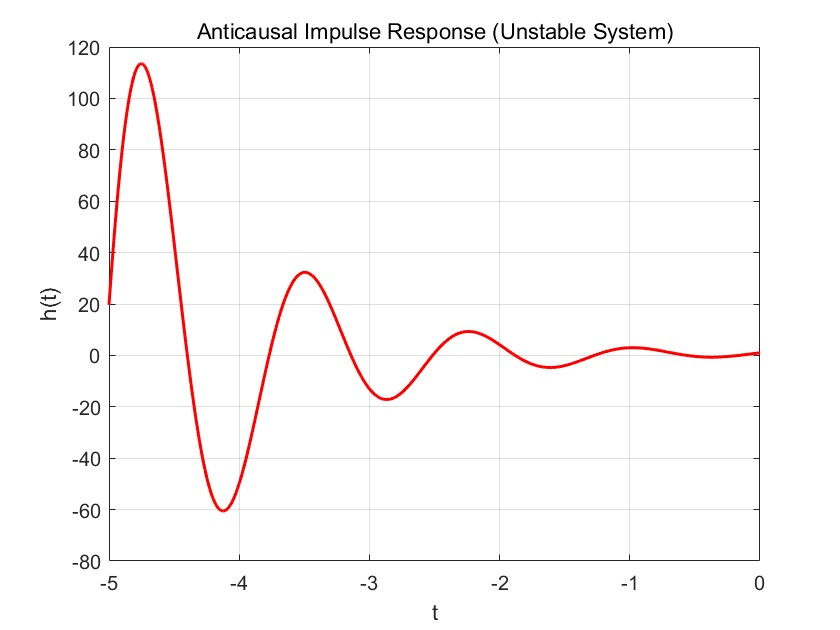
\includegraphics[width=0.5\textwidth]{36.jpg}
\end{figure}


\subsection*{(l)}

From the partial fraction expansion in part (i):
\[
H(s) = \frac{r_1}{s - p_1} + \frac{r_2}{s - p_2} + \frac{r_3}{s - p_3}
\]
where:
\begin{itemize}
    \item $p_1 \approx 1$ (right-half plane pole)
    \item $p_2, p_3 \approx -1 \pm j5$ (left-half plane poles)
\end{itemize}

For the stable system with ROC $-1 < \Re(s) < 1$, we decompose $H(s) = H_1(s) + H_2(s)$ where:
\[
H_1(s) = \frac{r_2}{s - p_2} + \frac{r_3}{s - p_3}, \quad \text{ROC: } \Re(s) > -1
\]
\[
H_2(s) = \frac{r_1}{s - p_1}, \quad \text{ROC: } \Re(s) < 1
\]

Thus $h_1(t)$ is causal and $h_2(t)$ is anticausal.

\subsection*{(m)}

\[
h_1(t) = r_2 e^{p_2 t} u(t) + r_3 e^{p_3 t} u(t)
\]
\[
h_2(t) = -r_1 e^{p_1 t} u(-t)
\]

The stable system's impulse response is $h_s(t) = h_1(t) + h_2(t)$.

\subsection*{(n)}
Combining the causal poles, $H_1(s)$ is a proper rational function with real coefficients:
\[
H_1(s) = \frac{b_2 s^2 + b_1 s + b_0}{s^2 + a_1 s + a_0}
\]

The corresponding differential equation is:
\[
\frac{d^2 y_1(t)}{dt^2} + a_1 \frac{d y_1(t)}{dt} + a_0 y_1(t) = b_2 \frac{d^2 x(t)}{dt^2} + b_1 \frac{d x(t)}{dt} + b_0 x(t)
\]

\textbf{Auxiliary conditions:} Initial rest conditions. For a second-order system:
\[
y_1(t_0^-) = 0,\quad y_1'(t_0^-) = 0
\]

\subsection*{(o)}

For $H_2(s) = \dfrac{r_1}{s - p_1}$ with ROC $\Re(s) < p_1$:
\[
\frac{d y_2(t)}{dt} - p_1 y_2(t) = r_1 x(t)
\]

\textbf{Auxiliary conditions:} Final rest conditions (since the system is anticausal):
\[
y_2(t_0^+) = 0
\]

\subsection*{(p)}

The input signal is:
\[
x(t) = \begin{cases}
1, & -3 \leq t \leq 2 \\
0, & \text{otherwise}
\end{cases}
\]

For the causal part $H_1(s)$, the output $y_1(t)$ is computed directly using numerical integration with initial rest conditions.

For the anticausal part $H_2(s)$, the output $y_2(t)$ is obtained via time reversal:
\begin{enumerate}
    \item Define the time-reversed input $r(t) = x(-t)$.
    \item The time-reversed system is causal: $\displaystyle H_{\text{rev}}(s) = -\frac{r_1}{s + p_1}$.
    \item Compute $w(t)$ as the response of $H_{\text{rev}}(s)$ to input $r(t)$ using initial rest conditions.
    \item Obtain $y_2(t) = w(-t)$.
\end{enumerate}

The total output of the stable noncausal system is:
\[
y(t) = y_1(t) + y_2(t)
\]

The simulation is performed on the interval $-10 \leq t \leq 10$ with time samples. The following plots are generated:
\begin{itemize}
    \item Input $x(t)$: a rectangular pulse from $t = -3$ to $t = 2$.
    \item $y_1(t)$: output of the causal subsystem.
    \item $y_2(t)$: output of the anticausal subsystem.
    \item $y(t) = y_1(t) + y_2(t)$: total output of the stable noncausal system.
\end{itemize}

This parallel realization allows numerical simulation of the stable LTI system despite its noncausal nature.

\begin{figure}[H]
\centering
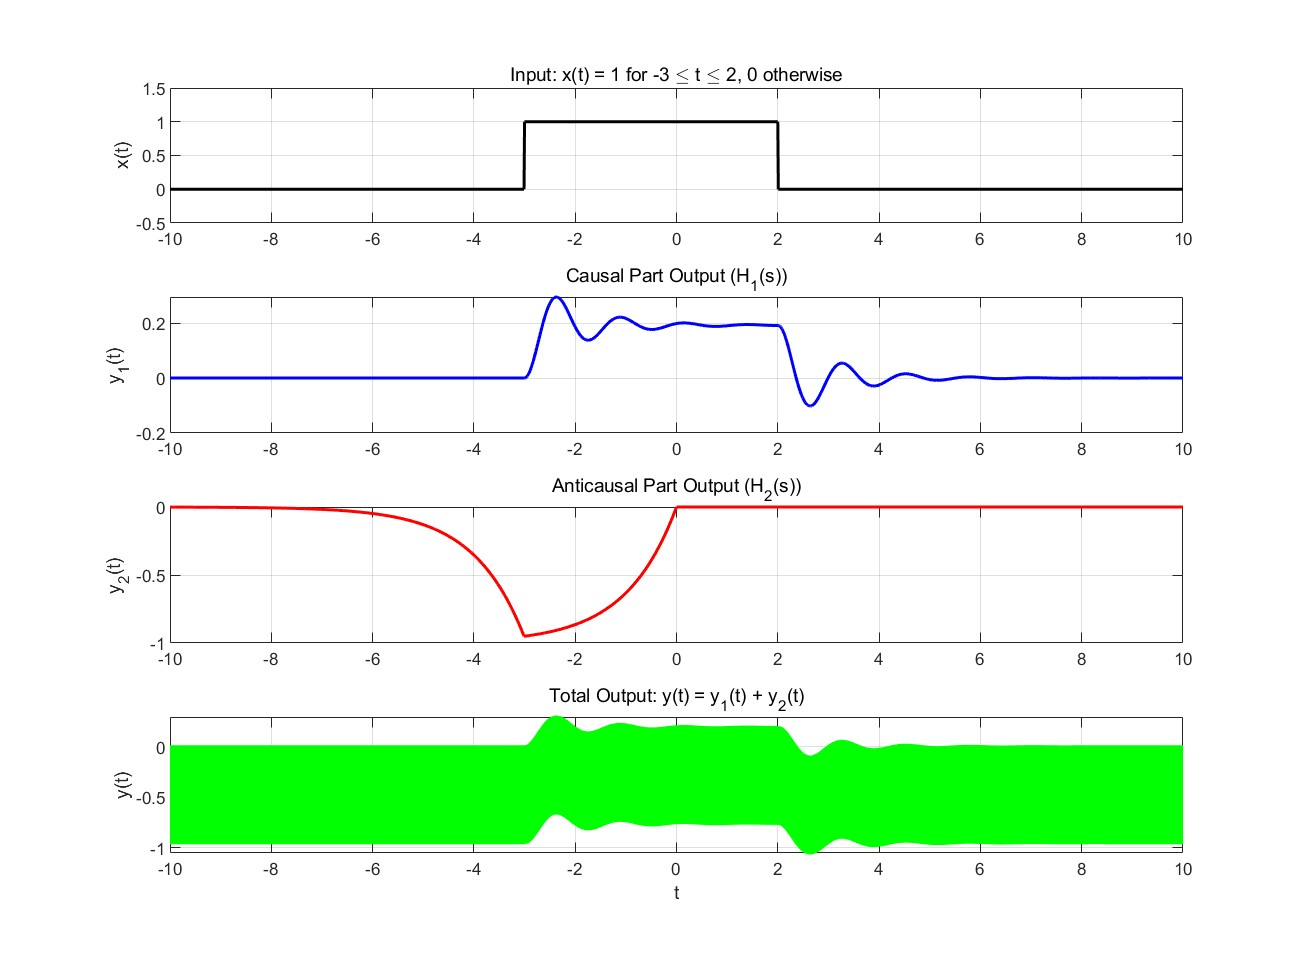
\includegraphics[width=1\textwidth]{37.jpg}

\end{figure}

\end{document}